\documentclass[UTF8,a4paper,10pt,nocolorlinks]{ctexart}
% \documentclass[UTF8]{ctexart}
\usepackage[left=2.50cm, right=2.50cm, top=2.50cm, bottom=2.50cm]{geometry} %页边距
\CTEXsetup[format={\Large\bfseries}]{section} %设置章标题居左   


\usepackage{setspace}
\usepackage{xcolor}
\usepackage{mdframed}
\usepackage{titletoc}
\usepackage{etoolbox}
%%%%%%%%%%%%%%%%%%%%%%%
% -- text font --
% compile using Xelatex
%%%%%%%%%%%%%%%%%%%%%%%
% -- 中文字体 --
%\setmainfont{Microsoft YaHei}  % 微软雅黑
%\setmainfont{YouYuan}  % 幼圆    
%\setmainfont{NSimSun}  % 新宋体
%\setmainfont{KaiTi}    % 楷体
%\setmainfont{SimSun}   % 宋体
%\setmainfont{SimHei}   % 黑体
% -- 英文字体 --
%\usepackage{times}
%\usepackage{mathpazo}
%\usepackage{fourier}
%\usepackage{charter}
\usepackage{helvet}
\usepackage{caption}
\usepackage{multicol} %用于实现在同一页中实现不同的分栏
\usepackage{changepage}
\usepackage{graphics}
\usepackage{amsmath, amsfonts, amssymb} % math equations, symbols
\usepackage[english]{babel}
\usepackage{color}      % color content
\usepackage{graphicx}   % import figures
\usepackage{url}        % hyperlinks
\usepackage{bm}         % bold type for equations
\usepackage{multirow}
\usepackage{booktabs}
\usepackage{epstopdf}
\usepackage{epsfig}
\usepackage{algorithm}
\usepackage{algorithmic}
\newcommand{\sihao}{\fontsize{14pt}{\baselineskip}}
\renewcommand{\algorithmicrequire}{ \textbf{Input:}}     % use Input in the format of Algorithm  
\renewcommand{\algorithmicensure}{ \textbf{Initialize:}} % use Initialize in the format of Algorithm  
\renewcommand{\algorithmicreturn}{ \textbf{Output:}}     % use Output in the format of Algorithm  
\renewcommand{\figurename}{图}
% 引用参考文献标号显示在右上角
\newcommand{\upcite}[1]{\textsuperscript{\textsuperscript{\cite{#1}}}}
% \hypersetup{colorlinks=false} 
% \usepackage{fancyhdr} %设置页眉、页脚
% %\pagestyle{fancy}
% \lhead{}
% \chead{}
% %\rhead{\includegraphics[width=1.2cm]{fig/ZJU_BLUE.eps}}
% \lfoot{}
% \cfoot{}
% \rfoot{} 
\usepackage{color}
\usepackage{subfigure}
\usepackage{changepage}
\usepackage{fancyhdr} %设置页眉、页脚
%双线页眉的bai设置


\pagestyle{fancy}  %%%单线页眉
\fancyhead{}
\fancyhead[LO]{Research on UAV scheduling technology based on big data platform}
\fancyhead[RO]{fengxuewei}
% \fancyfoot[RO]{\thepage}
\fancypagestyle{plain}{%
  \pagestyle{fancy}
}
\usepackage{shorttoc}
\usepackage{xcolor}
\usepackage{mdframed}
\usepackage{titletoc}
\usepackage{lipsum}

\renewcommand{\today}{\CJKnumber\year 年 \CJKnumber\month 月 \CJKnumber\day 日}

\DeclareRobustCommand{\chuhao}{\fontsize{42pt}{\baselineskip}\selectfont}  % 初号
\DeclareRobustCommand{\xiaochu}{\fontsize{36pt}{\baselineskip}\selectfont} % 小初
\DeclareRobustCommand{\yihao}{\fontsize{26pt}{\baselineskip}\selectfont}   % 一号
\DeclareRobustCommand{\xiaoyi}{\fontsize{24pt}{\baselineskip}\selectfont}  % 小一
\DeclareRobustCommand{\erhao}{\fontsize{22pt}{\baselineskip}\selectfont}   % 二号
\DeclareRobustCommand{\xiaoer}{\fontsize{18pt}{\baselineskip}\selectfont}  % 小二
\DeclareRobustCommand{\sanhao}{\fontsize{16pt}{\baselineskip}\selectfont}  % 三号 
\DeclareRobustCommand{\xiaosan}{\fontsize{15pt}{\baselineskip}\selectfont} % 小三
\DeclareRobustCommand{\sihao}{\fontsize{14pt}{\baselineskip}\selectfont}   % 四号
\DeclareRobustCommand{\xiaosi}{\fontsize{12pt}{\baselineskip}\selectfont}  % 小四
\DeclareRobustCommand{\wuhao}{\fontsize{10.5pt}{\baselineskip}\selectfont} % 五号
\DeclareRobustCommand{\xiaowu}{\fontsize{9pt}{\baselineskip}\selectfont}   % 小五
\DeclareRobustCommand{\liuhao}{\fontsize{7.5pt}{\baselineskip}\selectfont} % 六号
\DeclareRobustCommand{\xiaoliu}{\fontsize{6.5pt}{\baselineskip}\selectfont}% 小六
\DeclareRobustCommand{\qihao}{\fontsize{5.5pt}{\baselineskip}\selectfont}  % 七号
% \titlecontents{lsection}
%   [5.8em]{\sffamily}
%   {\color{secnum}\contentslabel{2.3em}\normalcolor}{}
%   {\titlerule*[1000pc]{.}\contentspage\\\hspace*{-5.8em}\vspace*{5pt}%
%     \color{white}\rule{\dimexpr\textwidth-15.5pt\relax}{1pt}}

% \newcommand\PartialToC{%
% \begin{mdframed}[backgroundcolor=ptcbackground,hidealllines=true]
% \printcontents[chapters]{l}{1}{\colorbox{ptctitle}{%
%   \parbox[t]{\dimexpr\textwidth-2\fboxsep\relax}{%
%     \strut\color{white}\bfseries\sffamily\makebox[5em]{%
%       Chapter~\thechapter\hfill}Contents}}\vskip5pt}
% \end{mdframed}%
% }
% \addcontentsline{toc}{section}{参考文献} %向目录中添加条目,以章的名义
% \pretocmd{\tableofcontents}{\begin{mdframed}[backgroundcolor=ptcbackground,hidealllines=true]}{}{}
% \apptocmd{\tableofcontents}{\end{mdframed}}{}{}
% \patchcmd{\tableofcontents}{\contentsname}{\color{ptctitle}\contentsname}{}{}

\providecommand{\keywords}[1]{\textbf{\textit{keywords---}} #1}
%%%%%%%%%%%%%%%%%%%%%%%
%  设置水印
%%%%%%%%%%%%%%%%%%%%%%%
%\usepackage{draftwatermark}         % 所有页加水印
%\usepackage[firstpage]{draftwatermark} % 只有第一页加水印
% \SetWatermarkText{Water-Mark}           % 设置水印内容
% \SetWatermarkText{\includegraphics{fig/ZJDX-WaterMark.eps}}         % 设置水印logo
% \SetWatermarkLightness{0.9}             % 设置水印透明度 0-1
% \SetWatermarkScale{1}                   % 设置水印大小 0-1    
 
\usepackage{hyperref} %bookmarks
% \usepackage[colorlinks,linkcolor=red,anchorcolor=blue,citecolor=green,CJKbookmarks=True]{hyperref}
\hypersetup{colorlinks, bookmarks, unicode} %unicode
 
 
 
\title{\textbf{基于大数据平台的无人机技术研究概述}}
\author{ 冯学伟\hspace{1em}学号:2019520941}
% \date{\today}
\date{2020年5月20日}
\begin{document}
    \maketitle
    \newcommand\blfootnote[1]{%
      \begingroup
      \renewcommand\thefootnote{}\footnote{#1}%
      \addtocounter{footnote}{-1}%
    \endgroup
    }
    \blfootnote{姓名:冯学伟}
    \blfootnote{学号:2019520941}
    \blfootnote{指导教师:孙靖宇}
    % 设置figure的下标显示 为"图"
  %   \begin{figure}[t]
	% 	\parbox[b]{2cm}{
	% 		
\includegraphics[width=\textwidth]{TYUT.jpg}
	% 		}
  % \end{figure}
  
% 	\begin{center}
% 		\quad \\
% 		\quad \\
% 		\heiti \fontsize{45}{17} 课\quad 程\quad 论\quad 文
% 		\vskip 3.5cm	
%         \begin{center}
%             \huge{\textbf{BP神经网路在UAV中的应用}}\\[3mm]
%             \Large{\textbf{Application of BP neural network in UAV}}\\[1mm]
%         \end{center}
% 	\end{center}
% 	\vskip 3.5cm

%     % \begin{quotation}
%         \begin{center}
%             % \begin{flushleft}
%             \songti \fontsize{15}{15}
%             \doublespacing
%             \par\setlength\parindent{12em}
%             \quad
%             \sanhao\par
%             学\hspace{1cm}  院:\underline{\qquad 软件学院 \quad} 

%             专\hspace{1cm}  业:\underline{\qquad 软件工程 \quad} 

%             学生姓名:\underline{\qquad 冯学伟 \qquad }     

%             学\hspace{1cm} 号:\underline{\quad 2019520941\quad}

%             指导教师:\underline{\qquad 冯秀芳 \qquad}
%             \vskip 2cm
%             \centering
%             \date{2020年5月20日}
%             % \end{flushleft}
%         \end{center}
%     % \end{quotation}
    
%     \thispagestyle{empty} % 设置当前页 页版式
%     \clearpage

%     \captionsetup[figure]{labelfont={bf},labelformat={default},labelsep=period,name={图}}

%      % 目录
%     \renewcommand{\contentsname}{目录}  % 将Contents改为目录
%     \tableofcontents
%     % \tableofcontents
%     % \tableofcontents
%      % empty: 无页眉页脚
%      % plain: 无页眉,页脚为居中页码
%      % headings: 页眉为章节标题,无页脚
%      % myheadings: 页眉内容可自定义,无页脚
%     \thispagestyle{empty} % 设置当前页 页版式
%     \clearpage % 分页/

    \begin{adjustwidth}{0cm}{0cm}
        \large{\textbf{摘\hspace{1em}要:}}无人机凭借其低成本、 高效率等优点, 正成为提升农业植保科技含量的重要装备。 针对目前无人机作业
资源调度不合理、 效率低下以及地主和飞服组织之间缺乏有效的沟通渠道等问题, 基于互联网大数据云平台对
无人机调度技术进行了研究。 该平台一共分为 5 层, 分别为数据采集层、 网络传输层、 平台层、 访问层、 用户层。
根据不同用户的需求设计了不同的 APP, 分别为“我是地主” 和“我是飞手” , 为地主与飞服组织之间搭起了
沟通的桥梁, 实现了飞手和种植户的供需无缝对接。 以飞手为服务对象, 提出基于回溯策略的无人机调度算法,
在作业季内预计可提高飞手收益 20.1%。 实现了对无人机资源的高效调配。 将互联网技术融入植保无人机的作
业之中, 为实现农业信息化做出了有益的尝试
        \begin{flushleft}
        \par\textbf{关键字: } 无人机; 大数据;互联网; 调度平台 %“\par在段首,表示另起一行,“\textbf{}”,花括号内的内容加粗显示
        \end{flushleft}
    \end{adjustwidth}
  % adjustwidth \usepackage{changepage}
  \begin{adjustwidth}{0cm}{0cm}
      \large{\textbf{Abstract: }}The standard and high efficiency of the UAV itself are becoming important equipment for improving the scientific and technological content of agricultural plant protection. In view of the current unreasonable drone operation resource scheduling, low efficiency, and the lack of effective communication channels between the landlord and the flight service organization, the platform is divided into 5 layers, namely the data collection layer, network transmission layer, platform layer, and access layer , User layer. Different APPs have been designed according to the needs of different users, namely "I am the landlord" and "I am the flying hand", which establishes a coaxial communication between the landlord and the flying suit organization, realizing the flying hand and the grower's Seamless supply and demand. Taking the pilot as the service object, a drone scheduling algorithm based on the backtracking strategy is proposed, which is expected to increase the pilot’s income in the 20.1 industry during the operating season, making a useful attempt to realize agricultural informatization.
      % \noindent 首行缩进
  \end{adjustwidth}
  \begin{keywords}
      \noindent UAV, the big data, the Internet, the Dispatching platform  
  \end{keywords}
  \thispagestyle{empty} % 设置当前页 页版式
  \clearpage % 分页
    

\section{scala学习心得}
经历了几周的关于scala的学习,对编程的认知有更上了一个层次;下面我将就这一段时间的学习,来梳理出相关的学习内容:
\subsection{函数式编程(fp)、面向对象编程(OOP)、面向过程编程(POP)}
面向过程编程(POP)就是分析出解决问题所需要的步骤,然后用函数把这些步骤一步一步实现,使用的时候一个一个依次调用就可以了。面向对象编程(OOP)是把构成问题的事务分解成各个对象,建立对象的目的不是为了完成一个步骤,而是为了描述某个事物在整个解决问题的步骤中的行为。我们通过把大段代码拆成函数,通过一层一层的函数调用,就可以把复杂任务分解成简单的任务,这种分解可以称之为面向过程的程序设计。函数就是面向过程的程序设计的基本单元。\par
而函数式编程(Functional Programming),虽然也可以归结到面向过程的程序设计,但其思想更接近数学计算。我们需要先搞清楚计算机(computer)和计算(compute)的概念;在计算机的层次上,CPU执行的是加减乘除的指令代码,以及各种条件判断和跳转指令,所以,汇编语言是最贴近计算机的语言。而计算则指数学意义上的计算,越是抽象的计算,离计算机的硬件越远。对应到编程语言,就是越低级的语言,越贴近计算机,抽象程度低,执行效率高,比如C语言;越高级的语言,越贴近计算,抽象程度高,执行效率低,比如Lisp语言。\par
函数式编程就是一种抽象程度很高的编程范式,纯粹的函数式编程语言编写的函数没有变量,因此,任意一个函数,只要输入是确定的,输出就是确定的,这种纯虚数我们称之为没有副作用。而允许使用变量的程序设计语言,由于函数内部的变量状态不确定,同样的输入,可能得到不同的输出,因此,这种函数是有副作用的。函数式编程的一个特点就是,允许把函数本身作为参数传入另一个函数,还允许返回一个函数。\par
\subsection{Scala内置的数据结构}
Scala内置的数据结构包括数组、元组、容器、序列、集合、映射、迭代器等。
数组是一种可变的、可索引的、元素具有相同类型的数据集合;Scala提供了参数化类型的通用数组类Array[T],其中T可以是任意的Scala类型,可以通过显式指定类型或者通过隐式推断来实例化一个数组。关于数组的操作有声明数组、多维数组的创建、数组元素的使用等.\par
元组是对多个不同类型对象的一种简单封装。定义元组最简单的方法就是把多个元素用逗号分开并用圆括号包围起来。使用下划线$"_"$加上从1开始的索引值,来访问元组的元素,如果需要在方法里返回多个不同类型的对象,Scala可以通过返回一个元组来实现。\par
同时Scala提供了一套丰富的容器(collection)库,包括序列(Sequence)、集合(Set)、映射(Map)等,Scala用了三个包来组织容器类,分别是collection,mutable和immutablel; collection封装了可变容器和不可变容器的超类或特质,定义了可变容器和不可变容器的一些通用操作。\par
序列(Sequence)是一种内部元素可以按照特定的顺序访问的容器。序列中每个元素均带有一个从0开始计数的固定索引位置,序列容器的根是collection.Seq特质。其具有两个子特质 LinearSeq和IndexedSeq。LinearSeq序列具有高效的 head 和 tail 操作,而IndexedSeq序列具有高效的随机存储操作。实现了特质LinearSeq的常用序列有列表(List)和队列(Queue)。实现了特质IndexedSeq的常用序列有可变数组(ArrayBuffer)和向量(Vector)。\par
Scala内部存在于列表相对的数据结构---集合,集合(set)是不重复元素的容器(collection);而列表(List)中的元素是按照插入的先后顺序来组织的。“集合”中的元素并不会记录元素的插入顺序,而是以“哈希”方法对元素的值进行组织,所以,集合允许你快速地找到某个元素。\par
映射(Map)是一系列键值对的容器。键是唯一的,但值不一定是唯一的。可以根据键来对值进行快速的检索。 Scala 的映射包含了可变的和不可变的两种版本,分别定义在包mutable 和immutable 里。默认情况下,Scala中使用不可变的映射。如果想使用可变映射,必须明确地导入mutable.Map。若想要获取映射中的值,可以通过键来获取。\par
迭代器(Iterator)不是一个容器,而是提供了按顺序访问容器元素的数据结构,迭代器包含两个基本操作:next和hasNext。next可以返回迭代器的下一个元素,hasNext用于检测是否还有下一个元素。除next和hasnext方法外,在对一个迭代器调用了某个方法后,不要再次使用该迭代器。\par
\subsection{Spark运行架构特点}
每个Application获取专属的executor进程,该进程在Application期间一直驻留,并以多线程方式运行tasks。Spark Application不能跨应用程序共享数据,除非将数据写入到外部存储系统;Spark与资源管理器无关,只要能够获取executor进程,并能保持相互通信就可以了,Spark支持资源管理器包含: Standalone、On Mesos、On YARN、Or On EC2;提交SparkContext的Client应该靠近Worker节点(运行Executor的节点),最好是在同一个Rack(机架)里,因为Spark Application运行过程中SparkContext和Executor之间有大量的信息交换;如果想在远程集群中运行,最好使用RPC将SparkContext提交给集群,不要远离Worker运行SparkContext;Task采用了数据本地性和推测执行的优化机制,关键方法:taskIdToLocations、getPreferedLocations。
\subsection{RDD运行机制}
一个 RDD 就是一个分布式对象集合,提供了一种高度受限的共享内存模型,其本质上是一个只读的分区记录集合,不能直接修改。每个 RDD 可以分成多个分区,每个分区就是一个数据集片段,并且一个 RDD 的不同分区可以保存到集群中不同的节点上,从而可以在集群中的不同节点上进行并行计算。\par
在Spark中,转换的作用是从现有数据集创建新数据集。转换是惰性的,因为它们仅在动作需要将结果返回到驱动程序时才计算。Spark采用textFile()方法来从文件系统中加载数据创建RDD,该方法把文件的URI作为参数,这个URI可以是:本地文件系统的地址;或者是分布式文件系统HDFS的地址;或者是Amazon S3的地址等等.\par
RDD操作包含转换操作、行动操作和惰性机制。对于RDD而言,每一次转换操作都会产生不同的RDD,供给下一个“转换”使用,转换得到的RDD是惰性求值的,也就是说,整个转换过程只是记录了转换的轨迹,并不会发生真正的计算,只有遇到行动操作时,才会发生真正的计算,开始从血缘关系源头开始,进行物理的转换操作;行动操作是真正触发计算的地方。Spark程序执行到行动操作时,才会执行真正的计算,从文件中加载数据,完成一次又一次转换操作,最终,完成行动操作得到结果;而所谓的“惰性机制”是指,整个转换过程只是记录了转换的轨迹,并不会发生真正的计算,只有遇到行动操作时,才会触发“从头到尾”的真正的计算。

\section{大数据相关技术介绍}
\subsection{Apache Hadoop 架构}
先来简要介绍 Apache Hadoop 架构、Hadoop 分布式文件系统(Hadoop 
Distributed Filesystem)DFS 和 MapReduce 并行编程模型。
\par Apache  Hadoop  是阿帕奇软件基金会的一个项目,它在 2005 年才逐渐成型,
虽然距离现在只过了短短 14 年,但它的发展却是日新月异的并逐渐开启了大数
据研究与应用的热潮。Hadoop 最大的特点是不管是老机器还是新机器都可以构
建 Hadoop 大数据平台,通过整合集群整体的存储和计算能力使其有更为强大的
计算和存储能力。Hadoop 的集群存储和多处备份的机制保证了它有很高的可靠
性,它可以在大数据运行的状态添加新机节点,这保证了它有很高的可伸缩性和
可扩展性。Hadoop 能方便的实现大数据批量处理,实现大规模数据的分布式存
储与并行计算。而且 Hadoop 是开源的,目前很多公司即使其使用者也是贡献者,
使 Hadoop 已成为非关系数据分析的主流技术。当然,关系数据库更容易使用,
特别是 SQL 语句,所以为了降低大数据的使用门槛很多人开始致力于大数据平
台上运行sql语句的研究如FaceBook为了在Hadoop集群上使用传统的sql语句,
而开发了 Hive。如图\ref{bigdata1}所示。
主要包括以下模块: 
\begin{itemize}
  \item [(1)] 
  Hadoop Common:支持其他 Hadoop 模块的常用实用程序。 
  \item [(2)]
  Hadoop 分布式文件系统(HDFS™):一种分布式文件系统,可提供对应用
程序数据的高吞吐量访问。
\item [(3)] 
Hadoop YARN:作业调度和集群资源管理的框架。
\item [(4)] 
Hadoop  MapReduce:基于 YARN 的系统,用于并行处理大型数据集
\end{itemize}

\begin{figure}[h]
  \centering % 图片居中
  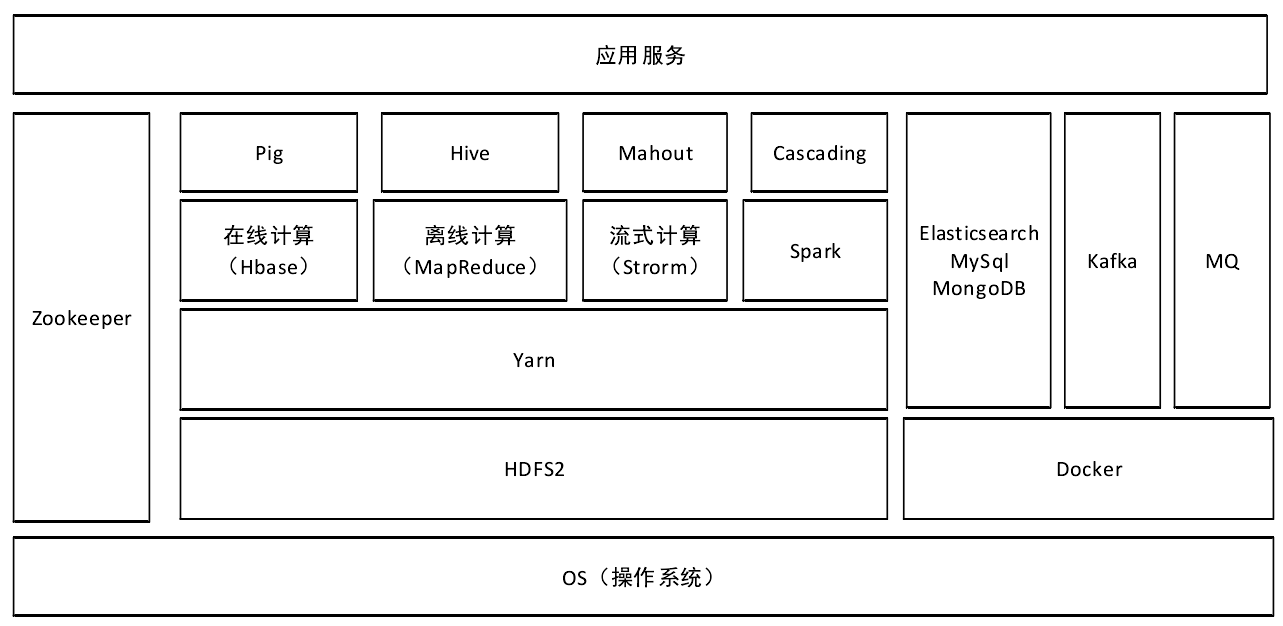
\includegraphics[width=0.8\textwidth]{bigdata_1.png} % 在命名上面也有要求??? 我靠
  \caption{大数据平台架构图}
  \label{bigdata1}
\end{figure}

从图中可以看出在操作系统之上是 Hadoop 的 HDFS 分布式文件存储系统,
yarn 在其上作为 Hadoop  资源管理器,它是一个通用资源管理系统,可为上层应
用提供统一的资源管理和调度。在 yarn 的上面可以运行像 MapReduce  、spark、
Habse、Stom、Pig、Hive、Mahout 等多种分布式计算。ZooKeeper 字面意思是
动物管理员,而 pig、hive 又都是各种动物的名字,所有从名字就可以看出
ZooKeeper 是来管理和协调各种分布式应用的,可以使分布式应用更方便的进行
分布式计算,在 Hadoop 中发挥着举足轻重的作用。不过不管是哪一种分布式
计算,它们所使用的计算的基本思想都是 MapReduce。下面我们重点介绍一下
MapReduce 并行编程模型。\par 
MapReduce 是一个编程模型。谷歌首先提出将其作为大规模数据处理的并行
计算模型和方法。它用于大规模数据集(大于 1TB)并行计算。Hadoop 诞生
于谷歌在国际会议上发表的两篇关于谷歌分布式文件系统和 MapReduce 的论文
[30]。其中 Map 译为映射,其实就是把任务进行拆分,把不同的任务分别配给不
同的机器去执行。Reduce 译为归约其实就是把运算的结果进行进一步的计算再
进行合并得到最终结果,其原理图如图\ref{bigdata2}所示: 
\begin{figure}[h]
  \centering % 图片居中
  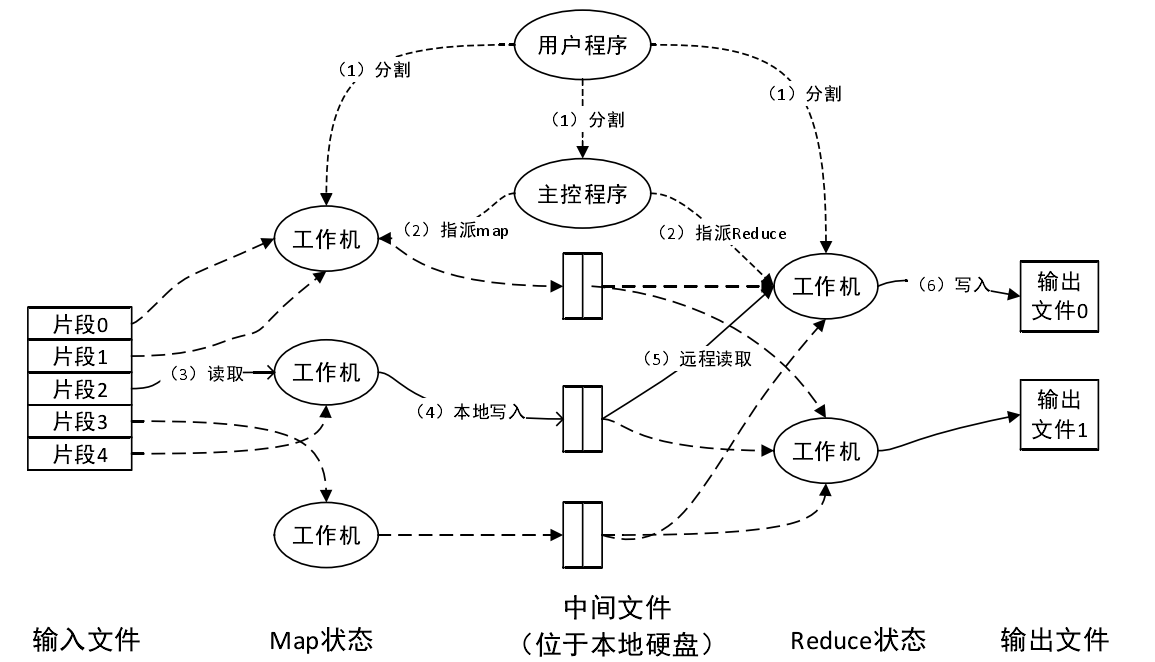
\includegraphics[width=0.8\textwidth]{bigdata_2.png} % 在命名上面也有要求??? 我靠
  \caption{MapReduce 原理图}
  \label{bigdata2}
\end{figure}
\par 当向大数据平台提交 MapReduce 任务后,首先主控程序也就是 Master 会向
把任务分配给工作机(slave),然后数据被分成多个片段分配给不同的工作机,
工作机再对数据进行各种处理并把处理结果先写入工作机的本地磁盘中,然后再
有 1 到 2 个工作机把处理结果进行汇总,再输出就是处理完成后的结果了。
\subsection{Spark 架构}
Apache Spark 诞生于 2009 年,因为 Hadoop 虽然开创了大数据开发的先河,
但其启动慢,计算也慢,虽然听过增加集群的规模可以提高运算速度,但仍不尽
如人意。为了克服 Hadoop 的缺点,在 2009 年 Spark 就诞生了,它作为一种新的
集群计算系统,以其飞快的速度迅速就引起了研究和应用的热潮,它提供 Java,
Scala,Python 和 R 中的高级 API,以及支持通用执行图的优化引擎。它还支
持一组丰富的更高级别的工具,包括 Spark SQL 用于 SQL 和结构化数据的处理,
MLlib 机器学习,GraphX 用于图形处理和 Spark  Stream 用于流式数据的实时处
理。\par
Spark 用到了一种被称为 RDD(Resilient Distributed Datasets)的数据集,这
是一种弹性分布式数据集,Spark 拥有丰富的 RDD 算子可以让用户像处理本地
数据一样处理 Spark 大数据,因为 RDD 算子的丰富性可以让其处理大数据的方
式更为灵活,并且避免了冗余的 MapReduce 操作,和冗余的磁盘 IO 通过缓存到
内存,多线程执行等操作保证了 Spark 运算的速度。Spark  是在  Scala  语言中实
现的,与 Hadoop 不同,Spark 和 scala 可以紧密集成,scala 可以像本地收集对象
一样轻松地操作分布式数据集。虽然 Spark 是为支持分布式数据集上的迭代作
业而创建的,但它实际上是 Hadoop 的补充,可以在 Hadoop 文件系统上运行。
\par Spark 计算模型具有速度快、使用方便、统一分析引擎的优势。
    \section{基于大数据平台的无人机调度技术研究}
    无人机作为技术成熟、 性能稳定的工具, 服务
越来越智能、 高效、 精准, 而当无人机与物联网、
与农业有效融合时, 无疑将带来数据采集及应用的
巨大突破。 目前而言, 全美 65\% 的化学农药采
用飞机作业完成喷洒, 年处理 40\% 以上的耕地面积;
其中水稻施药作业 100\% 采用航空作业方式; 日本
有 60\% 的水稻田采用无人机飞防来完成防治的, 近
40\% 的农田植保防治是用无人机来完成的。 中国耕
地面积约为 1.33 亿 hm2, 按照 40\% 植保作业由植保
无人机完成, 则有 0.53 亿 hm2[ 4-5] 。 植保无人机在
2016 年以来, 整体市场和产品可靠性都得到长足的
发展。 从 2018 年的态势来看, 整个行业的销量有不
会低于 3 万台。 这样 1 个数字已经极大地超越了目
前政府可能补贴的极限。 这意味着整体用户市场开
始接受植保无人机作为 1 个作业工具, 承认它的效
果和效率。 随着无人机的普及, 无人机在农业
中也得到了广泛的应用, 逐渐暴露出以下问题: 一
是现在平台没有整合气象、 交通、 维修等信息, 没
有专门为农户、 飞服组织提供的个性化信息服务。
飞服公司没有 1 个合适的平台联系种植户, 出现了
“找活难” 的现象。 二是信息不对称, 在作业过程中,
面对海量的农田作业信息, 对于飞服组织而言, 通
常都是根据主观经验对选择的农田作业点进行调配,
依据经验或盲目地选择作业农田。 由于没有科学的
调配方案, 常常出现成本过高、 收益较少的问题。\par
在利用农业机械提升工作效率方面, 有许多学
者在不同的方面开展了广泛的研究。 文献[ 19] 提
出了 1 种基于机主选择的农机调配模式, 建立了以
高收入低成本为目标的优化模型, 实现了基于启发
式优先级规则的农机调配算法。 文献[ 20] 提出了
跨区域作业问题中带时间窗的农机调度问题, 提出
了基于智能智能遗传算法的农机调度策略。 本研究
是在张璠的农机跨区作业紧急调配算法适宜性选择
的基础上[ 21] , 提出了基于回溯策略的单机多任务
的无人机调度算法。 在无人机不足时, 基于最短距
离优先的紧急调配算法性能更加有优势。 在此算法
基础上, 结合回溯策略, 找到无人机作业的最优规
划路线, 是本研究的核心。 实现了飞手和种植户的
供需无缝对接, 为飞服组织提供最优益的调配方案,
具有重要的现实意义和应用价值\upcite{uav1}.


    % \begin{center}
    %     \large{\textbf{Abstract}}
    % \end{center}
    % % adjustwidth \usepackage{changepage}
    % \begin{adjustwidth}{0cm}{0cm}
    %     \hspace{1.5em} Due to the low cost and high efficiency, UAV is becoming an important equipment to improve agricultural 
    %     plant protection technology. Aiming at the problems of unreasonable resource scheduling, low efficiency and the lack 
    %     of effective communication channels between landlords and ★ying service organizations, a UAV(unmanned aerial 
    %     vehicle) scheduling system based on Internet big data cloud platform is proposed. The platform is divided into ■ve 
    %     layers (data acquisition layer, network transport layer, platform layer, access layer, and user layer). Two different
    %     APP named "I am a farmer" and "I am a flyer" are designed according to the needs of different users. APP provides a 
    %     bridge between landlords and ★y serving organizations, and seamlessly connects supply and demand between the ★yer 
    %     and the planter. Taking the ★yer as the object of service, this paper proposes an UAV scheduling algorithm based on 
    %     backtracking strategy. During the operating season, it is expected to increase the ★yer income by 20. 1%, realizing the 
    %     ef■cient deployment of UAV resources. The integration of Internet technology and plant protection UAV operation 
    %     has made a bene■cial attempt to realize agricultural informatization.
    %     \noindent\hspace{1.5em}Simply put, according to the given value and the actual output value to form a control deviation, the deviation is proportionally, integrally and differentially combined into a control quantity by a linear combination, and the controlled object is controlled. The conventional PID controller serves as a linear controller. \par
    %     % \noindent 首行缩进
    % \end{adjustwidth}
    % % 关键词 % \providecommand{\keywords}[1]{\textbf{\textit{Index terms---}} #1}
    % \begin{keywords}
    %     \noindent UAV, BP neural network, PID control          
    % \end{keywords}
    % \thispagestyle{empty} % 设置当前页 页版式
    % \clearpage % 分页

    \setcounter{page}{1}        %从下面开始编页,页脚格式为导言部分设置的格式

%     %%%%%%%%%%%%%%%%%%%%%%%% 分栏 %%%%%%%%%%%%%%%%%%
%     % \begin{multicols}{2}
    \subsection{系统的总体架构}
    平台自顶向下分为用户层、 访问层、 平台层、
网络传输层、 数据采集层 5 层结构。平台整体结构如\ref{struct}所示。
%     % 『h』当前位置。将图形放置在正文文本中给出该图形环境的地方。如果本页所剩的页面不够,这一参数将不起作用。
%     % 『t』顶部。将图形放置在页面的顶部。
%     % 『b』底部。将图形放置在页面的底部。
%     % 『p』浮动页。将图形放置在一只允许有浮动对象的页面上。
    \begin{figure}[h]
            \centering % 图片居中
            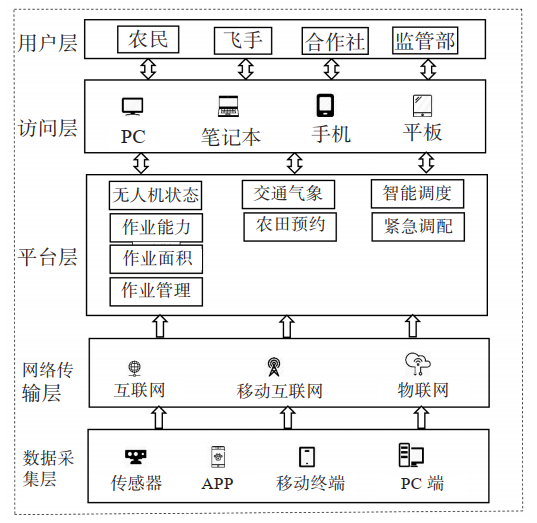
\includegraphics[width=0.5\textwidth]{struct.png} % 在命名上面也有要求??? 我靠
            \caption{系统结构图}
            \label{struct}
    \end{figure}
    \par 数据采集层: 大数据平台的数据采集来源主要
有飞手和农户自主发布的信息( 比如作物类型、 作
业时间窗、 作业报价、 面积等) 、 机载传感器向服
务器传送的数据( 比如无人机的位置等) 、 地图和
天气接口获取的相关信息。 机载传感器采集的数据
要求实时性强的数据适合采用物联网的方式自动获
取。\par
网络传输层: 基于有无人机作业的地点不固定,
环境多变等特性, 有一些数据要求实时性较高, 所
以将移动互联网作为机载数据传输方式是最适合的。
平台层: 在平台运行过程中, 会产生巨大的数
据量, Spark 是专业用于处理分布式存储的大数据工
具, 也非常适用于数据的低延迟访问以及对性能和
时间要求高的场景。 用户可以使用多种不同的终端
设备与大数据平台进行交互。\par
访问层: 由于终端的多样性, 使用 Web、 App
等技术实现用户界面和数据的展示。\par
用户层: 根据用户不同的需求, 设定不同的角色,
不同角色使用不同的 App。 “ 我是地主” 使用对象
是农民, “我是飞手” 使用对象是飞服公司。
\subsection{数据采集}
\subsubsection{机载数据单元采集数据}
数据采集的方式有
2 种, 分别是通过机载数据单元和客户端实现的。
机载数据单元由 GPS、 作业监控等若干传感器模块
组成, 采集来自北斗 /GPS 的无人机的地理位置信息、
作业情况等信息, 通过采集单元汇聚后经过移动无
线网络发送到平台的接收端, 采集到的数据发送到
智慧平台的数据库
\subsubsection{客户端采集数据}
客户端分为 $B/S$ 和 $App$ 2 种方式, 目的是为了满足不同用户在不同的使用
环境下的需求。 农民通过“ 我是地主” App 发布待
作业的农田信息, 包括: 单价, 地块面积等, 设定
农田中心点, 查询满足一定范围内的周边可用的无
人机进行作业。 
\subsection{调度算法}
智能调配要在时间期限内做出科学合理的决策,
规划出合理的调配方案。 无人机利用移动互联网、
北斗定位系统和物联网等信息技术, 为飞手和地主
提供智能决策与信息化服务, 提供收益最高的方案
规划。
智能调配要在时间期限内做出科学合理的决策,
规划出合理的调配方案。 无人机利用移动互联网、
北斗定位系统和物联网等信息技术, 为飞手和地主
提供智能决策与信息化服务, 提供收益最高的方案
规划, 相关算法可查看文献[23]。\par
为了进一步验证算法的性能, 该文献模拟了 5 组无人机调度数据, 通过基于回溯策略调度算法计
算出平均每台无人机在作业季内收益为 3 811.22 元。经过 5 次随机反复测试, 随机调度计算得出平均每
台无人机在作业季内收益为 3 173.372 元。 由此可见,以飞手为服务对象, 平均每台无人机在作业季内预
计可提高收益 20.1\%.\par
该文献最终得出的结论有:
\begin{itemize}
  \item [(1)] 
  基于于互联网的无人机调度平台利用机载数据
  单元以及手机客户端等多种终端, 提供线上线下服
  务, 实现飞手和种植户的供需无缝对接;
  \item [(2)]
  基于回溯策略的单机多任务无人机调度算法
  为飞服公司提供了 5 个最优候选方案, 并按收益最
  大、 成本最低依次排列, 与传统的随机调度相比,
  在作业季内每台无人机收益可预计提高 20.1\%
\end{itemize}
\section{基于气象大数据的天气预测的研究}
随着社会的发展,人们的出行方式也从步行,骑马,自行车,汽车,火车,
高铁,飞机等不断演进。在交通运输领域目前除了高
铁之外发展最为迅猛的就数无人机了,比如近年来京东、顺丰已经开始进行无人
机送货的尝试了。无人机相对于有人驾驶的飞机有很多先天性的优势。有人驾驶
的飞机必须配备生命系统,仪表盘、供氧系统、通讯、空调等,无人机只需配备
自动驾驶系统和通讯系统,结构简单、制造成本低。另外,由于精简了飞机上的
设备,使得重量降低,核载率更高,运营成本更低。  \par 对于偏远山区隔山跑死马,
无人机有着先天的优势。无人机运输要解决的一个核心问
题就输无人驾驶问题,而解决无人驾驶问题的一个关键问题是规划无人机的飞行
路径。 
本课题\upcite{weather}将聚焦在未来无人机飞行时可能遇到的路径规划问题作为研究对象。天空中没有实体化的路线和标志,而
且对于飞机来说,对飞行影响最大的因素就是天气根据雷一钧的《中国飞机失
事统计》一文可以看到从  事故中原因记载统计出:不详 3 起,人为失误 7 起,
恶劣天气 5 起,飞机故障 5 起, 如图\ref{reason}所示。
\begin{figure}[h]
  \centering % 图片居中
  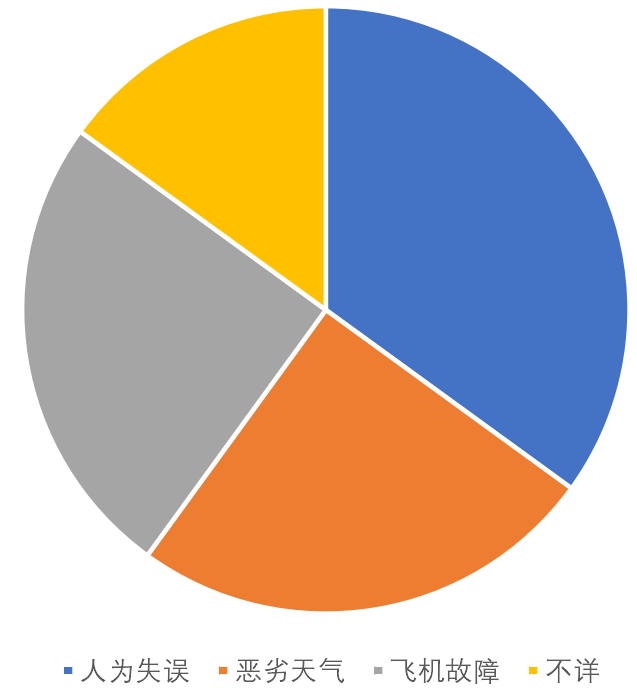
\includegraphics[width=0.5\textwidth]{reason.png} % 在命名上面也有要求??? 我靠
  \caption{失事原因}
  \label{reason}
\end{figure}
\par 可以看出恶劣天气对飞机坠毁的影响仅次于人为失误,排名第二位,如果使
飞行自动化,并避开恶劣天气,这样就解决了第一和第二两大飞机失事因素,极
大的增强飞行的安全性。因此我将研究如何规划无人机航线躲开天气恶劣的地区
使无人机能安全快速的到达目的地。基于现有气象大数据,通过机器学习处理的
方法准确预测天气,在此基础上规划无人运输飞行器的最佳路线,这将对未来无
人机运输有重要意义。 
\subsection{数据处理}
实验用到的数据来自天池大数据上的“未来已来——无人机路径优化大赛”
的比赛数据。赛事举办方称这些数据是来源伦敦气象局的真实数据,只是进行了
脱敏处理。提供的是 5 天的 20 多个 G 的 10 个模型的风力预测数据和相应的真
实天气数据。设计思路如下: \par
首先需要对原始的预测模型数据进行数据清洗,主要是一些缺失值和异
常值的清洗,该文中我们用中值滤波器对数据处理,以消除数据中的缺失值和异常
值的干扰。对于特征的提取主要是根据数据的实际意义,在原数据进行一番处理,得到
新的特征,一般情况下原数据的统计信息、方差等都有可能成为新的特征。最终我们用到的特征有:原始数据特征、
周围天气特征(上下左右)前后时间天气特征(前一个小时和后一个小时)、时
间特征(离散特征),平均值特征;其次就是在数据清洗之后进行分析。
\par
最后进行预测,预测方面可以有两种做法分类和回归。因为在最终规划路径的时候,我们会
把区域上的点,分为安全区域和危险区域,所以只要保证安全区域的点是安全的飞机可在安全区域自由航行,也就更有可能找到更短的路径。但是做回归的话虽
然可能找的安全区域系数更精确但在后续的路径规划的时候无人机飞行可能会
因为过度考虑飞行路线的安全性而绕了很远的路这样反而使油耗增加,而且在空
中呆的时间越久,那么在空中遇到危险天气的可能性也就越大,有点得不偿失。
在进行预测时我们还不得不考虑一下样本均衡问题,例如如当一天的天气很好时
大风区域会很小,或者某几天都是大风天,这样大风区域会很多,所以对于这样
的天我们采用随机抽样的方法,来使用样本更均衡。综合考虑这些因素,为了更
好的进行路径规划我们用二分类的方法作预测。\par
最后用数据结合各大预测模型,选取其中最优的几大预测方法得到的预测
F1 值(假定危险点为正例)对比
\subsection{处理流程}
本实验包括两部分,第一部分是进行天气预测,第二部分是进行无人能及航
迹规划,两者以前以后前者是后者的铺垫和前提。实验的整体数据处理流程图如
图\ref{flow}所示。 
\begin{figure}[h]
  \centering % 图片居中
  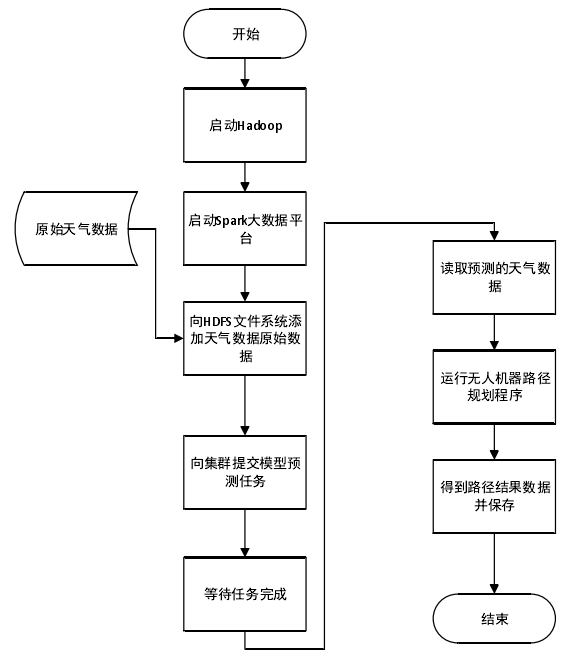
\includegraphics[width=0.8\textwidth]{DataFlow.png} % 在命名上面也有要求??? 我靠
  \caption{数据处理整体流程图}
  \label{flow}
\end{figure}
\par 由于本实验的均是在虚拟机上完成的,搭建的大数据平台的单机内存受到本
机内存的限制故而没有像真正的大数据平台那样拥有超大内存。所以本次实验并
没有使用全量的数据,只使用了从全量数据集中截取的 400 多兆的数据。

该文献把程序打包并提交集群任务和单机
任务进行对比实验,大数据集群对解决大数据运算的优势是可扩展性非常好,
如果处理的数据量增大,需求的时间短,增加相应的机器到集群中便增加了集
群的算力。对于无人机的路径规划算法,在基于传统 BFS 算法改造而得的时变的无人机路径规划算法和在此基础上结合 A*算法
添加路径评估函数,进一步改进而得的改进 BFS 算法和传统 BFS 进行比较,发
现在预测的准确率上面有了很大的提高。当然改进算法也有一点不足,在规划
出路径时用的时间有了一定的延长,但牺牲一点时间性能来获得路径代价的大
幅降低是值得的。通过实验验证了该天气预测模型和路径规划算法的可行性与
实用性和有效性。
\section{结论}
本文首先关于 Apache Hadoop, Spark, Habse、Stom、Pig、Hive、Mahout 等技术进行一定的介绍,其次主要就文献[23-24]展开详细的叙述,文献[23]主要介绍了大数据平台的无人机调度技术在农业方面的研究,
通过某种方式获取数据,输入到特定的算法内部借用大数据平台进行数据分析演算,从而可以验证该算法可以使得收益提高20.1\%,尽述了大数据平台的使用;文献[24]主要介绍了
基于气象大数据的天气预测,虽然已经有了很多研究方法可以借鉴,但每个方法都有它自身的局限性,故希望能综合使用各种预测方
法,让各种预测方法取长补短,使最后的预测结果更加符合本课题的需求。天气
预测一般包括风力、温度、湿度等多项指标的预测,由于文献[24]主要研究的天气数
据时要服务于无人机的路径规划,该无人机在空中飞行时影响其飞行的主要因素是风力,所以这里主要预测的是风力数据,最后通过在数据集合上应用该天气预测算法和路径规划算法并从时间效率
和飞行代价等方面对实验结果进行了对比分析,得出了可观的结论。\par
大数据平台在无人机领域的研究远远不止这两个方面,依然存在着很多大量的方向可以使得大数据和UAV更好地结合,对此需要我们不断深入学习,探索挖掘新思路。

%     BP(Back Propagation)神经网络分为两个过程:(1)、工作信号正向传递子过程 (2)、误差信号反向传递子过程;在BP神经网络中,单个样本有m个输入,有n个输出,在输入层和输出层之间通常还有若干个隐藏层。一个三层的BP网络就可以完成任意的m维到n维的映射。即这三层分别是输入层(I),隐含层(H),输出层(O)。其结构如图\ref{BP}所示。
%     \par 在BP神经网络中,输入层和输出层的节点个数都是确定的,而隐含层节点个数不确定,那么应该设置为多少才合适呢?实际上,隐含层节点个数的多少对神经网络的性能是有影响的,有一个经验公式可以确定隐含层    
%        节点数目,如下
%         \begin{equation} % 等式
%             h =\sqrt{m + n} + a \nonumber
%         \end{equation}
%     其中$h$为隐含层节点数目,$m$为输入层节点数目,$n$为输出层节点数目,$a$为1到10之间的调节常数。
%     % \subsection* 取消前面的标号


%     \subsection{正向传递子过程}
%     % $特殊符号表示$
%     现在设节点$i$和节点$j$之间的权值为 $\omega_{ij}$,节点$j$的阈值为$b_{j}$, 每个节点的输出值为$x_{j}$, 而每个节点的输出值是根据上层所有节点的输出值、当前节点与上一层所有节点的权值和当前节点的阀值还有激活函数来实现的.具体计算方法如下
%     \begin{equation} % 等式
%         % & 右对齐
%         \begin{aligned}
%         & S_j =\sum\limits_{i=1}^{m-1} \omega_{ij}x_{i} + b_{j} \nonumber \\
%         & x_{j}=f(S_{j})
%         \end{aligned}
%     \end{equation}
%     其中, $f$为激活函数, 一般选取$s$型函数或者线性函数。
%     正向传递的过程比较简单,按照上述公式计算即可。(在BP神经网络中,输入层节点没有阈值)
%     \subsection*{1.2 反向传递子过程}
%     在BP神经网络中,误差信号反向传递子过程比较复杂,它是基于Widrow-Hoff学习规则的。假设输出层的所有结果为$d_{j}$,误差函数如下
%     \begin{equation} % 等式
%         % & 右对齐
%         \begin{aligned}
%         & E(\omega, b) =\frac{1}{2}\sum\limits_{j=0}^{n-1}(d_{j} - y_{j}) ^ 2 \nonumber 
%         \end{aligned}
%     \end{equation}
%     而BP神经网络的主要目的是反复修正权值和阀值,使得误差函数值达到最小。

    
%     \section{BP神经网络PID控制器}
%     \begin{figure}[H]
%         \centering % 图片居中
%         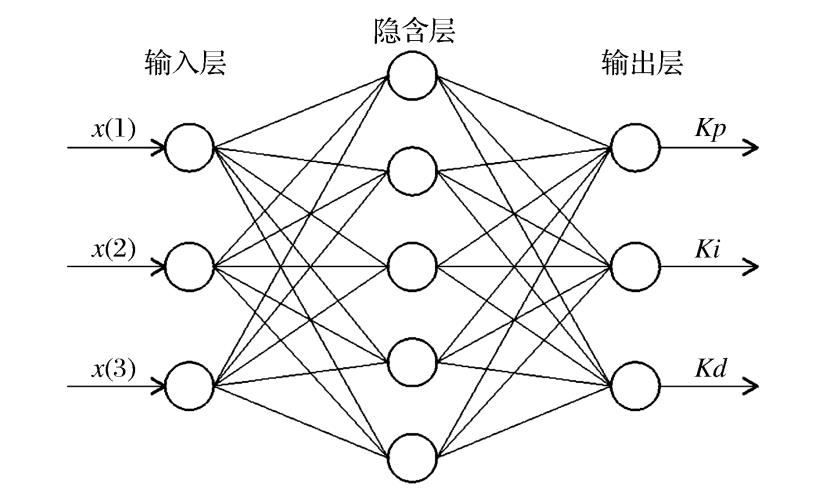
\includegraphics[width=0.7\textwidth]{PID_mode.jpg} % 在命名上面也有要求??? 我靠
%         \caption{PID控制神经网络}
%         \label{PID_BP}
%     \end{figure}
%     \subsection{改进型BP神经网络}
%     BP神经网络具有多层结构,包括输入层、隐含层和输出层,其中隐含层也可以是多层,具体与实际系统的训练程度相关,而且每一层都可以具有多个节点,也可以包含多个输入和输出值。在PID控制器的设计中,遇到的实际系统一般都是非线性的,采用BP神经网络算法可以通过梯度下降法来利用梯度搜索的技术使得
%     神经网络的实际输出值和我们期望的输出值的误差均方差降为最小。
%     \par 传统的BP神经网络在训练的时候,大都采用梯度下降法来求解权值和阈值,这种算法是先初始化一个解,然后在此基础上确定搜索方向和步长,这样初始解就会根据这个搜索方向和步长进行移动,从而使得待求解的目标函数输出下降,然后不断迭代下去,使得最后的误差比较小,在此过程中步长的选取显得尤为重要,
%     因为搜索算法确定之后整个求解过程都是基于此进行计算的,其运行过程是固定不变的,然而步长不一样,如果步长设置的过大,会使得搜索不仔细,可能引起系统的剧烈震荡,但是设置过小又会导致收敛速度太慢,从而达不到无人机控制系统快速性的要求,所以
%     步长的选定就会显得很重要了。学习率$/eta$就是用来对原步长进行调整的,但在传统的BP神经网络算法里它又是固定不变的,而研究将采取自适应改变学习率的方法,对其进行合理的调节,就是在训练误差比较大时,适当减小学习率,在训练误差比较小时,适当增加学习率,以期达到对传统BP神经网络算法来优化的目的。
%     根据整个系统的实时运行状态来不断调整权值系数, 不断学习, 使得输出层神经元的输出状态对应于 PID 控制器的 3 个参数 $K_{p}$ 、 $K_{i}$ 、 $K_{d}$ , 使其处于
%     实时变化中, 以此达到参数的在线整定 \upcite{6} 。当然这个变化是根据系统的运行状态而变,是一个动态调节的过程,而且最终的网络输出值也是在我们给定的某种最优化控制律下的参数,这样就实现了我们需要对整个无人机系统的自适应控制。
%     \par 采用3-5-3的神经网络结构,即输入层、隐含层、输出层分别含3个、5个、3个神经元的三层机构,如图\ref{PID_BP}所示。

%     \subsection{BP神经网络PID控制器算法}
%     BP神经网络输入神经元$M$ = 4;隐含层神经元$I$ = 5;输出神经元$J$ = 3,第m个输入神经元、第i个隐含层神经元、第j个输出神经元分别用$x_{m}$, $k_{i}$, $y_{j}$表示,$x_{m}$和$k_{i}$之间的权值为$\omega_{mi}$, $k_{i}$和$y_{j}$之间的权值$\omega_{ij}$。BP神经网络层采用正负对称的Sigmoid激活函数。由于网络输出$K_{p}$,$K_{i}$和$K_{D}$为负值,因此
%     输出层采用非负的Sigmoid激活函数\upcite{5},神经网络模型如图\ref{PID_BP}所示。\par
%     网络输入层的输入、输出为
%     \begin{equation} % 等式
%         % & 右对齐
%         \begin{aligned}
%         O_{m}^{(1)} =x_{m}(m=1,2,3,4)  
%         \end{aligned}
%     \end{equation}
%     \par 其中,$x_{1}$ = $r_{m}(k)$为系统的期望输入,$x_{2}$ = $y(k)$为系统的实际输入,$x_{3}$=$e(k)$,$x_{4}$=1为非线性调节的外部偏置常量。
%     网络隐含层的输入、输出为
%     % 分段函数
%     \begin{equation}
%         \begin{cases}
%         & net_{i}^{(2)}(k)=\sum\limits_{m=1}^{4}\omega_{mi}^{(3)}x_{m}\\
%         & O_{i}^{(2)}(k)=f(net_{i}^{(2)}(k)) \hspace{1em}(i=1,2,3,4,5)
%         \end{cases}
%     \end{equation}

%     网络输出层输入、输出为
%     \begin{equation}
%         \begin{cases}
%         & net_{j}^{(3)}(k)=\sum\limits_{i=1}^{5}\omega_{ij}^{(3)}(k)O_{j}^{(2)}(k)\\
%         & O_{j}^{(3)}(k)=g(net_{j}^{(3)}(k)) \hspace{1em}(j=1,2,3) \\
%         & O_{i}^{(3)}(k)=K_{P}, O_{2}^{(3)}(k)=K_{I}, O_{3}^{(3)}(k)=K_{D} g(net_{j}^{(3)}(k)) \hspace{1em}(j=1,2,3)
%         \end{cases}
%     \end{equation}
%     式中,$\omega_{mi}^{(2)}$、$\omega_{ij}^{(3)}$分别表示隐含层、输出层权值系数,上角标(1)、(2)、(3)分别表示输入层、隐含层、输出层。误差函数的选择根据梯度下降法的思想进行表达,取的性能指标函数为:
%     \begin{equation} % 等式
%         % & 右对齐
%         \begin{aligned}
%         E(k) =(r_{m}(k) - y(k))^2/2  
%         \end{aligned}
%     \end{equation}
%     以$\eta$为学习速率,$\alpha$为惯性系数的$\Delta\omega_{ij}^{(3)}$为:
%     \begin{equation}
%         \begin{cases}
%             % \partial导数符号
%             % 点乘:a \cdot b
%             % 叉乘:a \times b
%             % 除以:a \div b
%         & \Delta\omega_{ij}^{(3)}(k)=\eta\frac{\partial E(k)}{\partial \omega_{ij}^{(3)}(k)} + \alpha\Delta\omega_{ij}^{(3)}(k-1)  \sum\limits_{i=1}^{5}\omega_{ij}^{(3)}(k)O_{j}^{(2)}(k-1)\\
%         & \frac{\partial E(k)}{\partial \omega_{ij}^{(3)}(k)} = \frac{\partial E(K)}{\partial y(k)} \cdot{\frac{\partial y(K)}{\partial u(k)}} \cdot{\frac{\partial u(K)}{\partial O_j^{(3)}(k)}} \cdot{\frac{\partial O_j^{(3)}(k)}{\partial net_{j}^{(3)}(k)}} \cdot{\frac{\partial net_{j}^{(3)}(k)}{\partial \omega_{ij}^{(3)(k)}}}
%         \end{cases}
%         \label{con:formula1}
%     \end{equation}
%     用sgn($\frac{\partial y(k)}{\partial u(k)}$)代替$\frac{\partial y(k)}{\partial u(k)}$。由此带来的误差由学习速率$\eta$进行补偿:
%     \begin{equation}
%         \begin{cases}
%             % \partial导数符号
%             % 点乘:a \cdot b
%             % 叉乘:a \times b
%             % 除以:a \div b
%         & \frac{\partial net_{j}^{(3)(k)}}{\partial \omega_{ij}^{(3)(k)}} = O_{i}^{(2)}{k}, \frac{\partial u(k)}{\partial O_{i}^{(3)}(k)} = e(k) - e(k-1) = x_{1} \\
%         & \frac{\partial u(k)}{\partial O_{2}^{(3)}(k)} = e(k) = x_{2}, \frac{\partial u(k)}{\partial O_{3}^{(3)}(k)} = e(k) - 2e(k-1) = e(k-2) = x_{3}
%         \end{cases}
%     \end{equation}
%     式(\ref{con:formula1})可以写成:
%     \begin{equation}
%         \begin{cases}
%         & \Delta\omega_{ij}^{(3)}(k)=\alpha\Delta\omega_{ij}^{(3)}(k-1) + \eta\delta_{j}^{(3)}O_{j}^{(2)}(k) \\
%         & \delta_{j}^{(3)} = -\frac{\partial E(k)}{\partial net_{j}^{(3)}(k)} = e(k) \cdot{sgn(\frac{\partial y(k)}{\partial u(k)})} \cdot{\frac{\partial u(k)}{\partial O_{j}^{(3)}(k)}} \cdot{g'(net_{j}^{(3)}(k))}
%         \end{cases}
%     \end{equation}
%     同理:
%     \begin{equation}
%         \begin{cases}
%         & \Delta\omega_{mi}^{(2)}(k)=\alpha\Delta\omega_{mi}^{(2)}(k-1) + \eta\delta_{i}^{(2)}O_{m}^{(1)}(k) \\
%         & \delta_{i}^{(2)} = -\frac{\partial E(k)}{\partial net_{i}^{(2)}(k)} =f'(net_{i}^{(2)}) \cdot{\sum\limits_{j=1}^{3}\omega_{ij}^{(3)}(k)} \cdot{\delta_{j}^{(3)}}             e(k) \cdot{sgn(\frac{\partial y(k)}{\partial u(k)})} \cdot{\frac{\partial u(k)}{\partial O_{j}^{(3)}(k)}} \cdot{g'(net_{j}^{(3)}(k))}
%         \end{cases}
%     \end{equation}
%     \par 其中,$f(x)$=$e^{x}$-$e^{-x}$ / $e^{x}$ + $e^{-x}$, $g(x)$=$e^{x}$ / $e^{x}$ + $e^{-x}$。求导得$f'(x)$=(1-$f^{2}(x)$), $g'(x)$=2$g(x)$(1-$g(x)$)。
%     \clearpage % 分页
%     \section{结 论}
%     实验结果表明:BP神经网络阶跃响应速度较快,根据采样时间判断训练步数克制,BP神经网络在第39步时响应值为1.且无明显超调。传统的PID控制器也无明显超调,响应值在65步时才为1,由此可以证明,BP神经网络PID控制器比传统PID控制器响应快,实际应用中传统PID控制器要比此处的性能要差。
%     采用了两种PID控制方法:传统PID控制和BP神经网络PID控制.BP神经网络PID控制效果要明显
% 优于传统PID控制.传统PID控制器在不采用BP神经网络PID控制器训练过后的比例系数KP、微分系数
% KI、积分系数KD的情况下阶跃响应会产生较大幅度的超调和振荡,系统需要更长的时间才能稳定.传统
% PID控制器在采用BP神经网络PID控制器训练过后的比例系数KP、微分系数KI、积分系数KD的情况下阶
% 跃响应超调幅度降低,不会产生超调.BP神经网络PID控制阶跃响应迅速,且不会产生超调和振荡.改进
% 算法中的BP神经网络PID控制可以避免在快速响应的过程中产生超调和振荡,使系统更加稳定.
%     \clearpage % 分页
    
 
%     % \clearpage % 分页
%     % \section*{以下为一些工具}
%     %     \begin{align} % 对齐
%     %         & ABCDEFGHIJKLMNOPQRSTUVWXYZ \label{alphabet} \\
%     %         & abcdefghijklmnopqrstuvwxyz \\
%     %         & \alpha \beta \gamma \delta \epsilon \varepsilon \zeta \eta \theta \lambda \mu \nu \xi \pi \rho \sigma \tau \upsilon \phi \varphi \chi \psi \omega  
%     %     \end{align}

%     %     \begin{align}
%     %         % 不能使用 \[\] 标号来分割开下面三个
%     %         \begin{bmatrix}
%     %             1 & 2 \\
%     %             3 & 4 \\
%     %         \end{bmatrix}
%     %         \\
%     %         \begin{pmatrix}
%     %             1 & 2 \\
%     %             3 & 4 \\
%     %         \end{pmatrix}
%     %         \\
%     %         \begin{matrix}
%     %             1 & 2 \\
%     %             3 & 4 \\
%     %         \end{matrix}
%     %     \end{align}
    
%     %     \begin{equation} % 等式
%     %     A_{t+1} = \arg\min_A \ \mathcal{L}(A,E_t,\Delta\tau_t,W_t,b_t), \nonumber
%     %     \end{equation}
    
%     %     \begin{equation}
%     %         \begin{aligned} \label{eq:rasl}
%     %             \min_{A,E,\Delta \tau} \quad & \sum_{i=1}^{N}||A_i||_* + \lambda ||E_i||_1  \\
%     %             \mathrm{s.t.} \quad & D_i \circ \tau_i + \sum_{k=1}^{n_i} J_{ik} \Delta \tau_i \epsilon_k \epsilon_k^T = A_i + E_i, \\
%     %             & i = 1,2,\cdots,N. 
%     %         \end{aligned}
%     %     \end{equation}
    
%     %     % 标准表格的形式
%     %     \begin{table}[htbp]
%     %         \centering  % 显示位置为中间
%     %         \caption{standard table}  % 表格标题
%     %         \label{table1}  % 用于索引表格的标签
%     %         %字母的个数对应列数,|代表分割线
%     %         % l代表左对齐,c代表居中,r代表右对齐
%     %         \begin{tabular}{|c|c|c|c|}  
%     %             \hline  % 表格的横线
%     %             & & & \\[-6pt]  %可以避免文字偏上来调整文字与上边界的距离
%     %             1&2&3&4 \\  % 表格中的内容,用&分开,\\表示下一行
%     %             \hline
%     %             & & & \\[-6pt]  %可以避免文字偏上 
%     %             0.1&0.2&0.3&0.4 \\
%     %             \hline
%     %         \end{tabular}
%     %     \end{table}        

%     %     \begin{table}[htbp]
%     %         \caption{Title of table} \label{tab:table}
%     %         \centering
%     %         \addtolength{\tabcolsep}{-0mm} % 控制列间距
%     %         \begin{tabular}{ccccc}
%     %             \toprule[0.75pt]	% package booktabs
%     %             \multicolumn{4}{c}{table head} \\
%     %             \midrule[0.5pt]	% package booktabs
%     %             \multirow{4}{*}{text} & 1 & 2 & 3 & 4 \\  % package multirow
%     %             & 5 & 6 & 7 & 8 \\
%     %             \cmidrule[0.5pt]{2-4}	% package booktabs
%     %             & 9 & 10 & 11 & 12 \\
%     %             & 13 & 14 & 15 & 16 \\
%     %             \bottomrule[0.75pt]	% package booktabs
%     %         \end{tabular}
%     %     \end{table}

%     %     % \eqref{eq:alphabet} : eq:alphabet eq 代表的是公式
%     %     % \begin{figure}
%     %     %     \centering % 图片居中
%     %     %         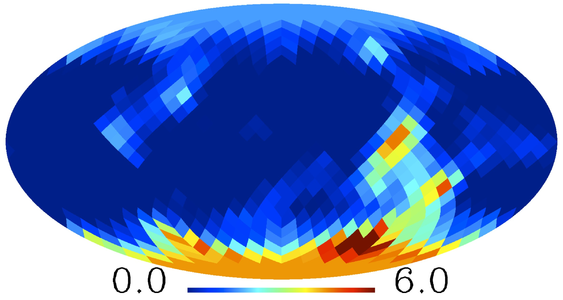
\includegraphics[width=\textwidth]{figure1.jpg}
%     %     %     \caption{摩擦角}
%     %     %     \label{fraction}
%     %     % \end{figure}
%     %     引用: Eq. \eqref{alphabet}, Fig. \ref{figure:fraction},  \\
%     %     \clearpage % 分页
        
%     % \end{multicols}
%         % 引用图片的时候, 要想引用成功, 必须要把标签加在图片命名之后:
    
%         % \begin{algorithm}
%         %     \caption{Title of the Algorithm}
%         %     \label{algo:ref}
%         %     \begin{algorithmic}[1]
%         %         \REQUIRE some words.  % this command shows "Input"
%         %         \ENSURE ~\\           % this command shows "Initialized"
%         %         some text goes here ... \\
%         %         % \WHILE {条件} 
%         %         \WHILE {\emph{not converged}}
%         %         \STATE ... \\  % line number at left side
%         %         \ENDWHILE
%         %         \RETURN this is the lat part.  % this command shows "Output"
%         %     \end{algorithmic}
%         % \end{algorithm}
%         % \clearpage % 分页
%         % plain,按字母的顺序排列,比较次序为作者、年度和标题.
%         % unsrt,样式同plain,只是按照引用的先后排序.
%         % alpha,用作者名首字母+年份后两位作标号,以字母顺序排序.
%         % abbrv,类似plain,将月份全拼改为缩写,更显紧凑.
%         % ieeetr,国际电气电子工程师协会期刊样式.
%         % acm,美国计算机学会期刊样式.
%         % siam,美国工业和应用数学学会期刊样式.
%         % apalike,美国心理学学会期刊样式.
%         % http://blog.sina.com.cn/s/blog_6fda97ea0102ycjp.html
%     % 文献引用
%     % \bibliographystyle{plain}
\clearpage
\addcontentsline{toc}{section}{参考文献}
\renewcommand{\refname}{参考文献}   % 将References改为参考文献
% % \cite{author1.year1,author2.year2}  “99” 表示以最多两位数来编号参考文献, 用于对齐
\begin{thebibliography}{99}
\addtolength{\itemsep}{-2ex} % 用于更改行距
% \bibitem{1}张岳平,朱力超,孙涛.用Hopfield神经网络与模拟退火算法求解UAV航路规划问题[J].海军航空工程学院学报,2007,22(4):451-453,466. DOI:10.3969/j.issn.1673-1522.2007.04.012.
% \bibitem{2}陈侠,艾宇迪.应用改进神经网络的无人机三维航迹规划[J].电光与控制,2018,25(9):7-11. DOI:10.3969/j.issn.1671-637X.2018.09.002.
% \bibitem{3}缪永飞.多UAV联合搜救任务规划建模及优化方法研究[D].湖北:武汉理工大学,2017.
% \bibitem{4}苏续军,吕学志.BP神经网络模型在无人机系统故障预测中的应用分析[J].计算机应用与软件,2019,36(9):70-75. DOI:10.3969/j.issn.1000-386x.2019.09.013.
% \bibitem{5}张永振,苏寒松,刘高华,等.基于BP神经网络的PID控制器参数调整[J].南开大学学报(自然科学版),2018,51(3):26-30.
% \bibitem{6}高富强,李萍,张磊敏,等.基于BP神经网络整定的PID控制及其仿真[J].山东陶瓷,2017,40(3):27-31. DOI:10.3969/j.issn.1005-0639.2017.03.007.
% \bibitem{7}余后明,刘彦臣,郑士振,等.基于改进型BP神经网络的四旋翼控制系统[J].甘肃科学学报,2019,31(2):87-91. DOI:10.16468/j.cnki.issn1004-0366.2019.02.015.
% \bibitem{8}虞晓霞.无人机飞行姿态稳定控制技术研究[D].吉林:长春理工大学,2018.
% \bibitem{9}朱凯光,王昊,彭聪,张琼,范天姣,景春阳.基于BP神经网络的固定翼航空电磁线圈姿态校正[J].吉林大学学报(地球科学版),2020,50(01):252-260.
\bibitem{1}Foulds L R, Wilson J M. Scheduling operations for the
harvesting of renewable resources[ J] . Journal of
food engineering, 2005,70(3):281-292.
\bibitem{1} Basnet C B, Foulds L R, Wilson J M.Scheduling
contractors’farm-to-farm crop harvesting operations
[ J] .InternationalTransactions in Operational
Research.2006,13(1):1-15.
\bibitem{1} Alio, Van Oudheusden D. In field logistics planning for
crop harvesting [ J] . Engineering optimization, 2009,
41(2): 183-197.
\bibitem{1} Foulds L R. hay harvesting operations scheduling
subject to probabilistic activity duration and machine
failure [ J] .Journal of Agricaltural studies. 2004,
41(2): 183-189.
\bibitem{1} 董玉玲 . 浅谈植保无人机推广中存在的问题及对策
\bibitem{1} . 新疆农垦科技, 2016, 39(7):27-28.
\bibitem{1} 刘科, 马根众 . 山东省农用植保无人机应用现状及建
议[ J] . 山东农机化, 2017(3):26-27.
\bibitem{1} 孔令亮 , 陆金晶 . 农业植保无人机发展现状浅析[ J] .
江苏农机化 ,2018(5):43-45
\bibitem{1} 胡善君 . 浅谈计算机在植保无人机系统中的应用[ J] .
科技创新与应用, 2017(13):49.
\bibitem{1} 蔡银杰 , 孙娟 , 丁晓辉 , 等 . 我国植保无人机发展现状
与展望[ J] . 世界农药 ,2018,40(6):15-18+36.
\bibitem{1} 胡冲 . 农机调配可视化系统研究[ D] . 保定: 河北农
业大学 ,2012.
\bibitem{1} 王春山 , 张璠 , 滕桂法 , 等 . 智慧农机调配管理平台设
计与实现[ J] . 中国农机化学报 ,2018,39(1):61-68.
\bibitem{1} 张璠 . 农机调配策略研究[ D] . 保定: 河北农业大
学 ,2012.
\bibitem{1} 王国新 , 宁汝新 , 王爱民 , 等 . 基于仿真的调度规则组
合决策研究[ J] . 北京理工大学学报 ,2006,26(7):38-
41+69.
\bibitem{1} 易平 , 李建军 , 熊禾根 . 基于多级优先规则的模具企业
动态车间作业调度算法[ J] . 模具工业 ,2009,35(5):7-9.
\bibitem{1} 郭鹏程 . 植保无人机调度平台的设计[ J] . 山西科
技 ,2018,33(1):74-76.
\bibitem{1} 张燕 , 滕桂法 , 王春山 , 等 . 基于 Android 手机的农机
调配系统[ J] . 农机化研究 ,2014,36(1):214-218.
\bibitem{1} 胡冲 , 吴焕瑞 , 滕桂法 , 等 . 农机调配多目标综合决策
检验[ J] . 农机化研究 ,2013,35(3):46-49.
\bibitem{1} 周三琦 . 农村信息化中农机调配策略及调配算法研究
[ D] . 郑州: 河南大学 ,2016.
\bibitem{1} 张璠 , 滕桂法 , 马建斌 , 等 . 基于启发式优先级规则的
农机调配算法[ J] . 农业工程学报 ,2012,28(10):78-85.
\bibitem{1} 王雪阳 , 苑侗侗 , 苑迎春 , 等 . 带时间窗的农机调度方
法研究[ J] . 河北农业大学学报 ,2016,39(6):117-123.
\bibitem{1} 张璠 , 滕桂法 , 苑迎春 , 等 . 农机跨区作业紧急调配算
法适宜性选择[ J] . 农业工程学报 , 2018, 34(5):47-53
\bibitem{uav1} 王昀,滕桂法.基于大数据平台的无人机调度技术研究[J].河北农业大学学报,2019,42(6):134-138. DOI:10.13320/j.cnki.jauh.2019.0134.
\bibitem{weather}李建平. 基于气象大数据的无人机航线规划研究与应用[D]. 北京工业,2019
\end{thebibliography}  

\end{document}